% !TEX encoding = UTF-8 Unicode
\documentclass[12pt,a4paper]{report}
 
\usepackage[brazil]{babel}
\usepackage[utf8]{inputenc}
\usepackage[T1]{fontenc}
\usepackage{graphicx, subfigure}
\usepackage{listings}
\usepackage{color}
\usepackage{mathtools}
\usepackage{indentfirst}

\definecolor{mygreen}{rgb}{0,0.6,0}
\definecolor{mygray}{rgb}{0.5,0.5,0.5}
\definecolor{mymauve}{rgb}{0.58,0,0.82}

\lstset{ %
  backgroundcolor=\color{white},   % choose the background color; you must add \usepackage{color} or \usepackage{xcolor}
  basicstyle=\footnotesize,        % the size of the fonts that are used for the code
  breakatwhitespace=false,         % sets if automatic breaks should only happen at whitespace
  breaklines=true,                 % sets automatic line breaking
  captionpos=b,                    % sets the caption-position to bottom
  commentstyle=\color{mygreen},    % comment style
  deletekeywords={...},            % if you want to delete keywords from the given language
  escapeinside={\%*}{*)},          % if you want to add LaTeX within your code
  extendedchars=true,              % lets you use non-ASCII characters; for 8-bits encodings only, does not work with UTF-8
  frame=single,                    % adds a frame around the code
  keywordstyle=\color{blue},       % keyword style
  language=Octave,                 % the language of the code
  morekeywords={*,...},            % if you want to add more keywords to the set
  numbers=left,                    % where to put the line-numbers; possible values are (none, left, right)
  numbersep=5pt,                   % how far the line-numbers are from the code
  numberstyle=\tiny\color{mygray}, % the style that is used for the line-numbers
  rulecolor=\color{black},         % if not set, the frame-color may be changed on line-breaks within not-black text (e.g. comments (green here))
  showspaces=false,                % show spaces everywhere adding particular underscores; it overrides 'showstringspaces'
  showstringspaces=false,          % underline spaces within strings only
  showtabs=false,                  % show tabs within strings adding particular underscores
  stepnumber=2,                    % the step between two line-numbers. If it's 1, each line will be numbered
  stringstyle=\color{mymauve},     % string literal style
  tabsize=2,                       % sets default tabsize to 2 spaces
  title=\lstname                   % show the filename of files included with \lstinputlisting; also try caption instead of title
}
\renewcommand*{\lstlistingname}{Exemplo}

\graphicspath{ {images/} }

\title{Solução para captura de análise de sinais analógicos}
\author{Mateus Ribeiro\\
	11/0017480\\
	mateusrba@gmail.com
	\and
	Vitor Vieira\\
	11/0067151\\
	vitor.ecomp@gmail.com
	\and
	Tiago Lenza\\
	11/0020987\\
	tiago.sk8@gmail.com
	\and
	Matheus Pedreira\\
	11/0017749\\
	matrpedreira@gmail.com
	\and
	Daniel Sandoval\\
	09/0109899\\
	daniel@loopec.com.br}
	
\begin{document}
\maketitle
\tableofcontents

\chapter{Introdução}

Sinais analógicos são extremamente importantes de serem analisados pois estes são a base para todos os sistemas de telecomunicações, além de nos fornecerem diversas informações sobre fenômenos naturais, tendo em vista que o sinal é uma onda variando no tempo. Um bom exemplo é o som.

Conseguir captar esses sinais analógicos nos possibilita analisá-los de diversas formas dependendo da aplicação. Um exemplo é a análise do som, que é uma vibração no ar, onde podemos separar diferentes sons pelas suas respectivas frequências.

\section{Objetivos}

Nosso objetivo principal ao procurar uma solução para captura de análise de sinais analógicos, era desenvolver uma solução móvel, de baixo custo, que pudesse ser utilizada sem grandes dificuldades, com uma precisão aceitável, e que tivesse uma aplicação real.

Também tínhamos como objetivo que a nossa solução fosse capaz de analisar a frequência do nosso sinal recebido para...

%Objetivo de analisar

Como um sinal analógico pode representar diversas informações diferentes, procuramos desenvolver cálculos de integral por barra e por trapézio que pudessem ser carregados na solução móvel para facilitar o cálculo da integral do sinal quando esse o fosse necessário.

\section{Sinais Analógicos}

Um sinal analógico é uma onda variável que representa uma medida variando em função do tempo, estes sinais normalmente são utilizados em contexto elétrico, no entanto, também podem estar em um contexto mecânico, pneumático hidráulico e em muitos outros pois qualquer informação pode ser convertida em um sinal analógico.

Sinais analógicos podem ser usados para medir mudanças em fenômenos físicos como o som, a luz, a temperatura, a posição ou a pressão através de um transdutor de sinal, este têm basicamente a função de converter energia de uma forma para outra. 

A principal vantagem em se utilizar um sinal analógico é a boa definição deste sinal pois ele possui uma quantidade infinita de resoluções, comparando com sinal digital percebemos que este possui uma maior densidade e robustez.

A principal desvantagem na utilização de sinais analógicos é a quantidade de ruído presente.

\subsection{Transmissão de Dados}

Para realização da transmissão de dados, é muito mais interessante transmitir um sinal analógico do que um digital. Visto que o dado analógico é mais robusto, ele está menos suscetível à interferências. Uma outra vantagem na utilização de sinais analógicos para transmissão é a capacidade de fácil processamento, o que barateia o custo de transmissão. Para que um sinal digital seja enviado na forma analógica, este deve ser modulado.

\chapter{Projeto de Hardware}

Nosso objetivo em hardware é captar um sinal elétrico analógico para análise. Para atingir o objetivo estabelecido, escolhemos a plataforma Arduino, baseada no microcontrolador ATmega328, para captar em sua entrata analógica o sinal e transmiti-lo via interface serial a um computador pessoal.

\section{Plataforma Arduino}

A plataforma Arduino de desenvolvimento de hardware consiste em uma placa de circuito impresso, ilustrada na Figura~\ref{fig:arduino}, e uma IDE - \textit{Integrated Development Environment} - que nos permite escrever código e programar o microcontrolador.

\begin{figure}[h]
\centering
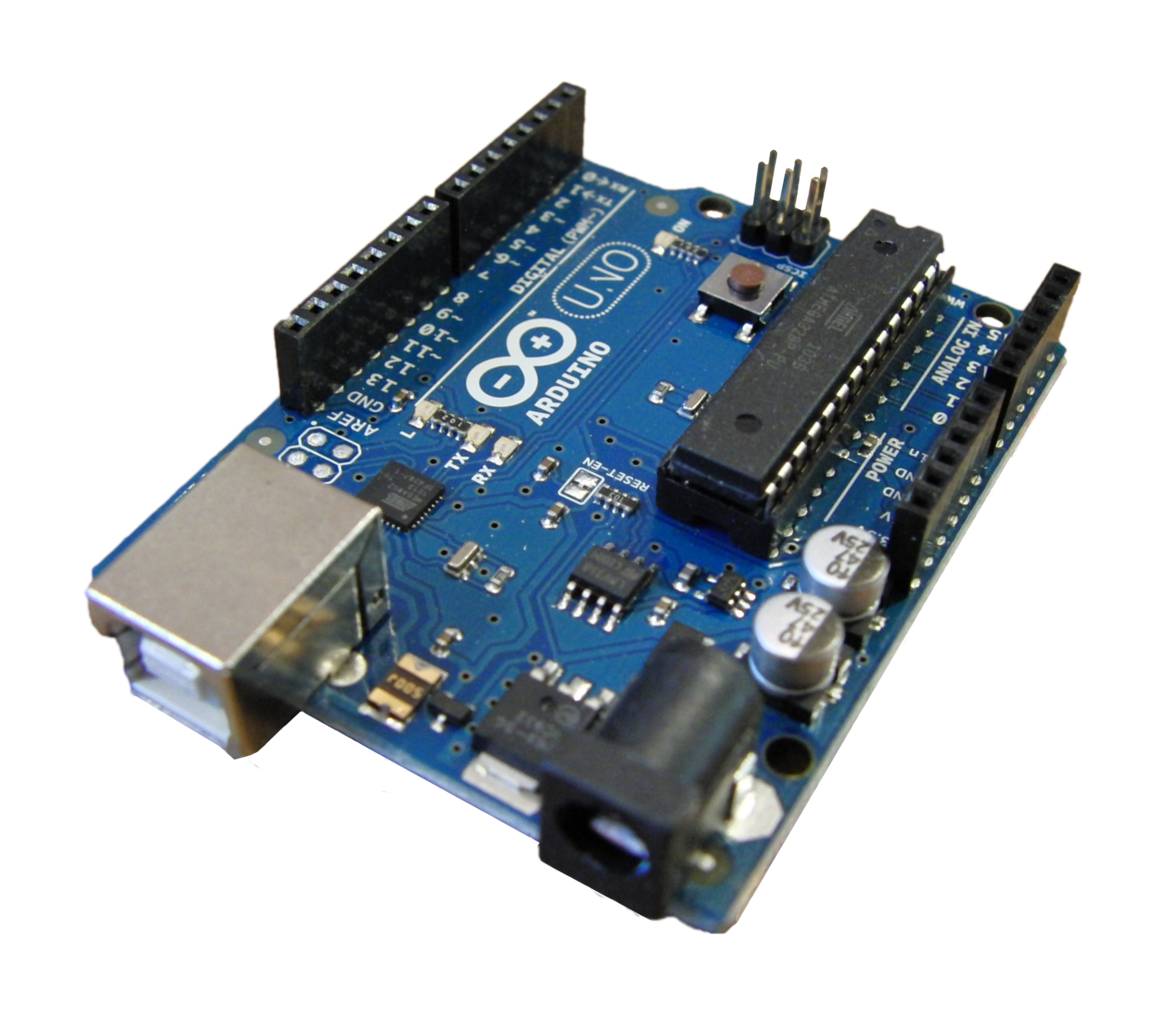
\includegraphics[width=0.7\textwidth]{arduino.png}
\caption{Arduino Uno}
\label{fig:arduino}
\end{figure}

No modelo utilizado da plataforma, o UNO, a placa de circuito impresso possui um microcontrolador ATmega382, que possui 2KB SRAM, 1KB EEPROM e opera a uma frequência máxima de 16MHz. Além do microcontrolador, estão presentes também alguns LEDs indicativos de estado, 13 pinos de comunicação digital e 6 entradas analógicas.

Utilizando a IDE fornecida, podemos codificar programas que interajam com os pinos digitais (que podem ser configurados como entrada ou saída), fazer leituras das entradas analógicas, e realizar computações sobre esses dados.

As bibliotecas fornecidas com o Arduino tornam a plataforma extremamente poderosa, capaz de cálculos matemáticos, operações com \textit{strings}, comunicação serial, entre outros.

\section{Metodologia e Desenvolvimento}

Como é possível visualizar no Exemplo~\ref{lst:arduino}, as bibliotecas disponíveis tornam a solução extremamente simples e elegante. Primeiramente, amostramos o sinal através da porta A0, armazenando o resultado no vetor de inteiros \textit{buffer}. A fim de se obter a máxima taxa de amostragem possível, são realizadas todas as leituras e armazenadas em memória, para que depois possam ser transferidas via interface serial.

A aquisição do sinal foi realizada detectando variações entre 0 e 5V representada em 1024 níveis (0-1023). Devido às limitações de memória da plataforma escolhida, nós podemos obter até 800 leituras a uma taxa \(470Hz\).

Segundo Teorema de Nyquist:

\begin{quotation}
“Para um sinal arbitrário de frequência \(B Hz\), o sinal da filtragem poderá ser completamente reconstruído pelo receptor caso a frequência de amostragem seja de no mínimo \((2B) Hz\).”
\end{quotation}

Portanto, temos que nossa solução de hardware é capaz de amostrar sinais com uma frequência de no máximo \(235Hz\).

Nosso projeto é capaz de identificar um sinal analógico elétrico a partir das entradas do Arduino, no entanto muitos dos sinais analógicos que são interessantes de serem analisados não estão em formato elétrico então a primeira coisa que deve ser feita antes de captar esses sinais é converte-los com o uso de transdutor, um exemplo dessa conversão é a leitura do som de um receptor como um microfone, após o som ser captado por este ele é convertido para o sinal analógico que será usado na nossa solução.

\lstinputlisting[language=C,caption={Código do Arduino},label={lst:arduino}]{code/arduino.c}

\chapter{Projeto de Software}

Nosso objetivo em software é analisar o sinal captado pela solução de hardware de maneira a identificar frequências presentes no sinal e suas respectivas magnitudes.

\section{Plataforma MATLAB}

A plataforma MATLAB (\textit{MATrix LABoratory}) é um software interativo de alta performance voltado para o cálculo numérico. O MATLAB integra análise numérica, cálculo com matrizes, processamento de sinais e construção de gráficos em ambiente fácil de usar onde problemas e soluções são expressos somente como eles são escritos matematicamente, ao contrário da programação tradicional.

Nossa escolha pela Plataforma MATLAB foi devido à agilidade no desenvolvimento, trazida por suas funções disponíveis e interfaces implementadas.

\section{Metodologia e Desenvolvimento}

Para realizar a análise do nosso sinal pela nossa solução de software é necessário primeiramente receber o dados que estão que foram adquiridos pelo Arduino. Esses dados são 800 números de 0 a 1023 e estão armazenados no vetor \textit{buffer} do microcontrolador.

\subsection{Transmissão do Sinal Adquirido}

Para transmissão dos dados adquiridos, utilizamos a interface serial, emulada de forma transparente sobre a interface USB. A transmissão ocorre da seguinte maneira, via interface serial, entre o Arduino e o computador:

\begin{enumerate}
\item [1.] Após a realização das 800 leituras, o Arduino fica em estado de espera;
\item [2.] O computador envia um caracter ao Arduino, solicitando uma leitura;
\item [3.] O Arduino envia ao computador a próxima leitura;
\item [4.] Os itens 2 e 3 se repetem até que sejam transmitidas as 800 leituras.
\end{enumerate}

\subsection{Análise do Sinal Adquirido}

A partir dos valores recebidos é possível realizar uma visualização gráfica do dados que nos ajuda a identificar o tipo do sinal, a forma da onda gerada por este sinal, o que, por sua vez, nos possibilita formular estratégias específicas para o tratamento do sinal que está sendo analisado.

Nossa solução computacional nos permite também analisar o sinal no domínio da frequência através de uma Transformada Rápida de Fourier, conhecida como FFT, que, por sua vez, é baseada na Série de Fourier.

A Série de Fourier, representada na Equação~\ref{eq:serie_fourier}, nos possibilita representar qualquer sinal através de um somatório de senos e cossenos.

\begin{equation}
f (t) = \frac{a_{0}}{2} + \sum_{n=1}^{\infty} [ a_{n}\cos{(\frac{n \pi t}{L})} + b_{n}\sin{(\frac{n \pi t}{L})} ]
\label{eq:serie_fourier}
\end{equation}

Uma vez obtida a representação em Série de Fourier do sinal original, os coeficientes \(a_{n}\) e \(b_{n}\) representam a magnitude de cada sinal periódico que o compõe.

A solução de software implementada aplica a Transformada Rápida de Fourier, que está disponível em biblioteca padrão do MATLAB, sobre o sinal original, obtendo os coeficientes \(a_{n}\) e \(b_{n}\) e provendo visualização gráfica da magnitude do sinal sobre o espectro da frequência.

Aplicações de analisar a frequência de um sinal:

\begin{itemize}
\item [-] Com o sinal no domínio da frequência é possível remover frequências indesejadas que podem ser geradas tanto por ruídos quanto por interferências, isso se aplica bem no caso de transmissões em redes de telecomunicação onde é possível saber como o sinal era para ter chegado para corrigi-lo caso necessário.
%\item [-]
\end{itemize}

\subsection{Integração}

\subsubsection{Integral Computacional}

\begin{figure}[h]
\centering
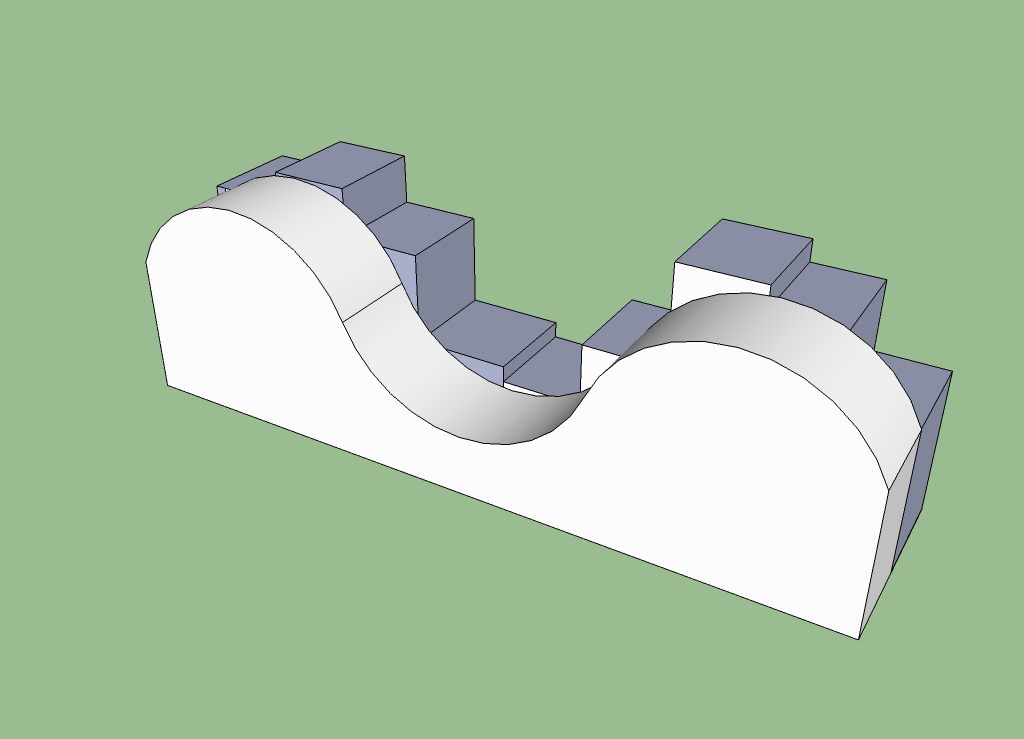
\includegraphics[width=0.7\textwidth]{integracao.png}
\caption{Integração computacional}
\label{fig:integracao}
\end{figure}

Método de integração computacional por somatório consiste em calcular de forma fixa uma parte da área do gráfico abaixo da função dada, e, após o cálculo, faz-se o somatório de todas as áreas. Quanto maior for a amostragem mais áreas serão calculadas fazendo com que o resultado da integral seja mais preciso, porém, com o aumento da amostragem, maior será o custo computacional. O cálculo da área abaixo da função pode ser feita de diversas formas, cada uma tendo suas vantagens em cada tipo de função, os métodos de cálculo de área implementados são:

\subsubsection{Trapézio}
É traçada uma reta entre dois pontos da amostra e através destes pode-se deduzir um trapézio, e através deste calcular a área entre os dois pontos do sinal. Esse tipo de somatório tem maior eficiência e precisão em sinais cuja a variação do sinal da derivada segunda, da função que representa o sinal, seja pequeno, ou seja funções apenas crescentes ou decrescentes.

\lstinputlisting[language=C++,caption={Integral por trapézio},label={lst:trapezio}]{code/trapezio.cpp}

\subsubsection{Por Barra}
É definido um ponto do sinal dentro do intervalo da amostragem, que é usado como o valor do sinal até o próximo ponto amostrado, fazendo com que cálculo da área seja maior ou menor do que o valor correto, porém em sinais cuja a variação do sinal da derivada segunda da função, que representa o sinal, seja alta e em funções periódicas mostra-se que a quantidade de área ganha acaba anulando a quantidade perdida, fazendo com que essa integral se saia melhor que a integral por trapézio neste tipo de função.

\lstinputlisting[language=C++,caption={Integral por barras},label={lst:barra}]{code/barra.cpp}

\subsubsection{Vantagens da integral por Somatório}
As grandes vantagens, do método por somatório, são a facilidade de implementação e a grande capacidade de paralelização deste processo em vários núcleos de processamento. Outra vantagem desse tipo de integração é a habilidade de não depender de uma função para o cálculo da integral sendo possível assim o cálculo direto de um sinal amostrado.

\chapter{Conclusão}

\subsection{Resultados Obtidos}

Os resultados obtidos foram de acordo com o esperado. Foi construída solução de hardware e software capaz de amostrar sinais elétricos a uma taxa de \(470 Hz\) e analisá-los no espectro da frequência. Conforme é possível constatar na Figura~\ref{fig:resultados}, a visualização gráfica dos sinais amostrados é extremamente satisfatória, bem como a visualização gráfica da distribuição de magnitude no espectro da frequência.

O software implementado para cálculo de integral funcionou corretamente e representa a possibilidade de melhora da solução, uma vez que foi implementado no formato de uma biblioteca de Arduino.

\subsection{Considerações Finais}

A solução desenvolvida em hardware e software representa ferramenta importante de análise de sinais analógicos. A possibilidade de integração em microcontroladores introduzida abre um leque imenso de aplicações sobre sinais analógicos em sistemas embarcados.

Através do desenvolvimento do projeto, verificou-se inclusive a importância do estudo de sinais analógicos, principalmente no âmbito do eletromagnetismo, importantíssimo para evolução de diversas tecnologias como, por exemplo, as de telecomunicações.

\begin{figure}[ht!]
     \begin{center}
        \subfigure[]{
            \label{fig:onda_seno}
            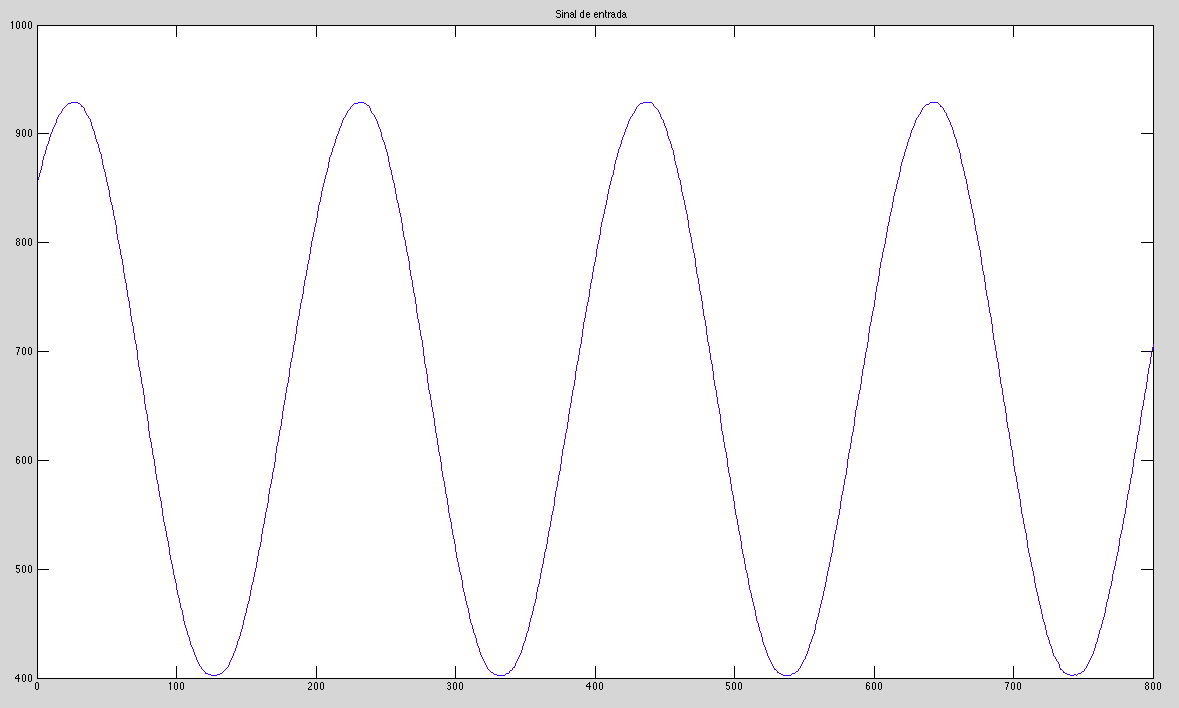
\includegraphics[width=0.47\textwidth]{seno.png}
        }
        \subfigure[]{
           \label{fig:onda_seno_fft}
           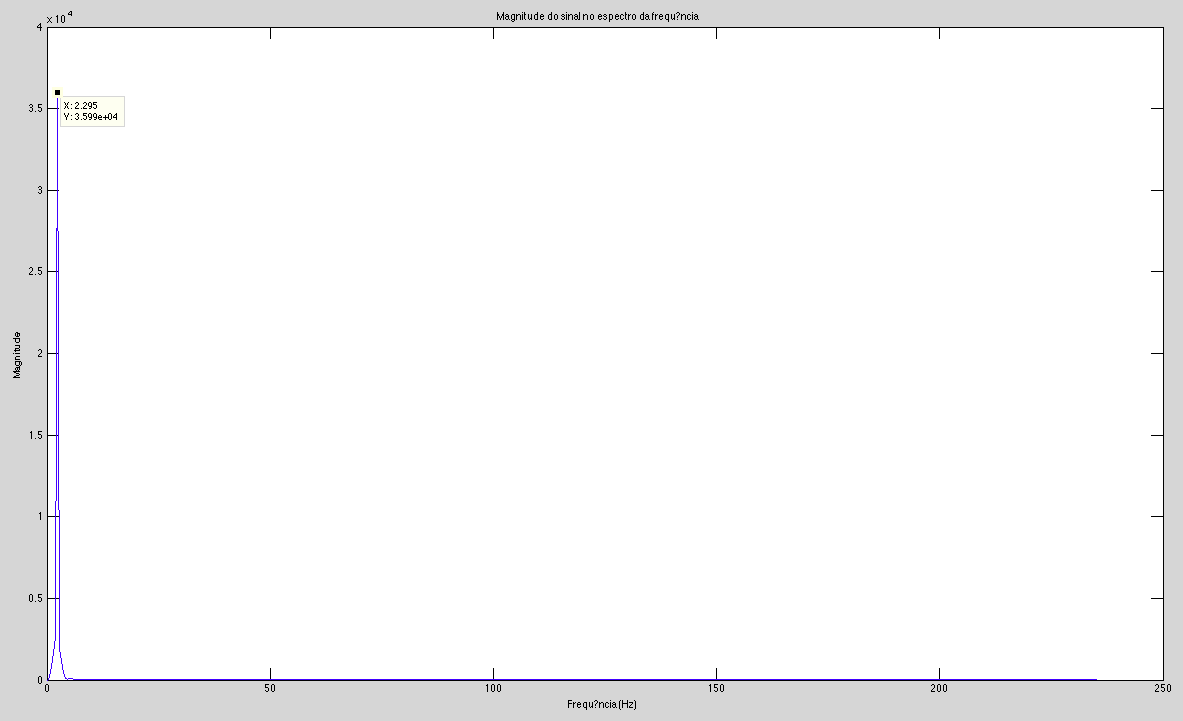
\includegraphics[width=0.47\textwidth]{seno_fft.png}
        }\\
        \subfigure[]{
            \label{fig:onda_triangular}
            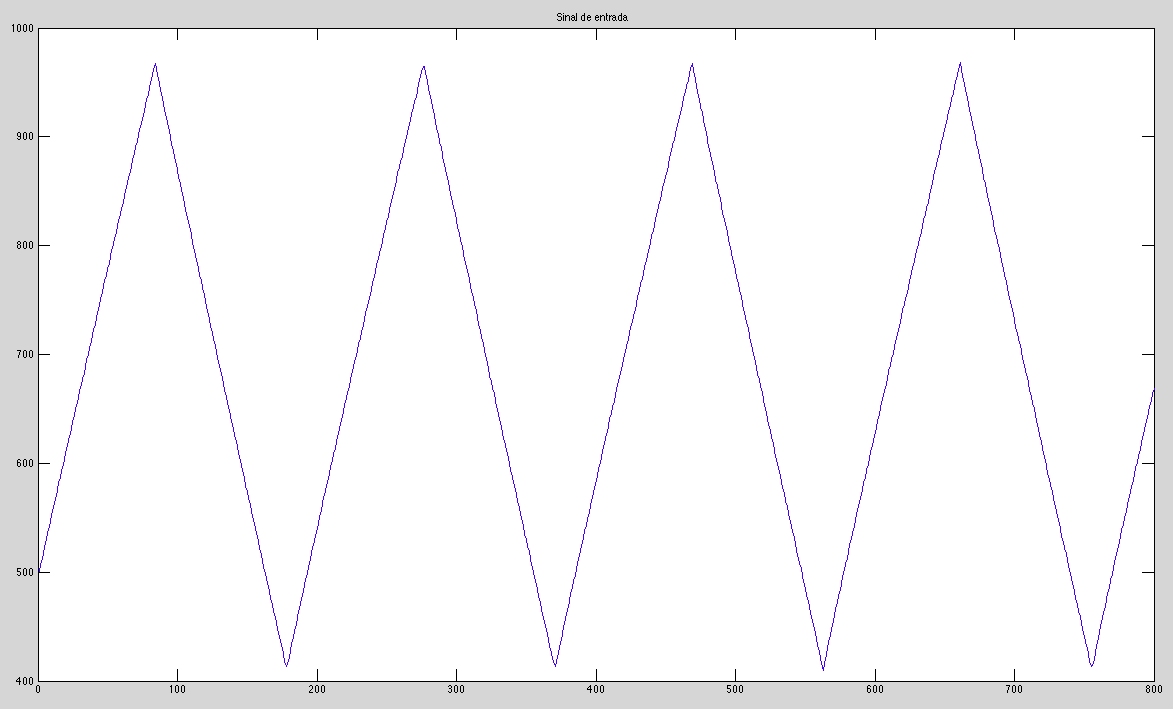
\includegraphics[width=0.47\textwidth]{triangular.png}
        }
        \subfigure[]{
            \label{fig:onda_triangular_fft}
            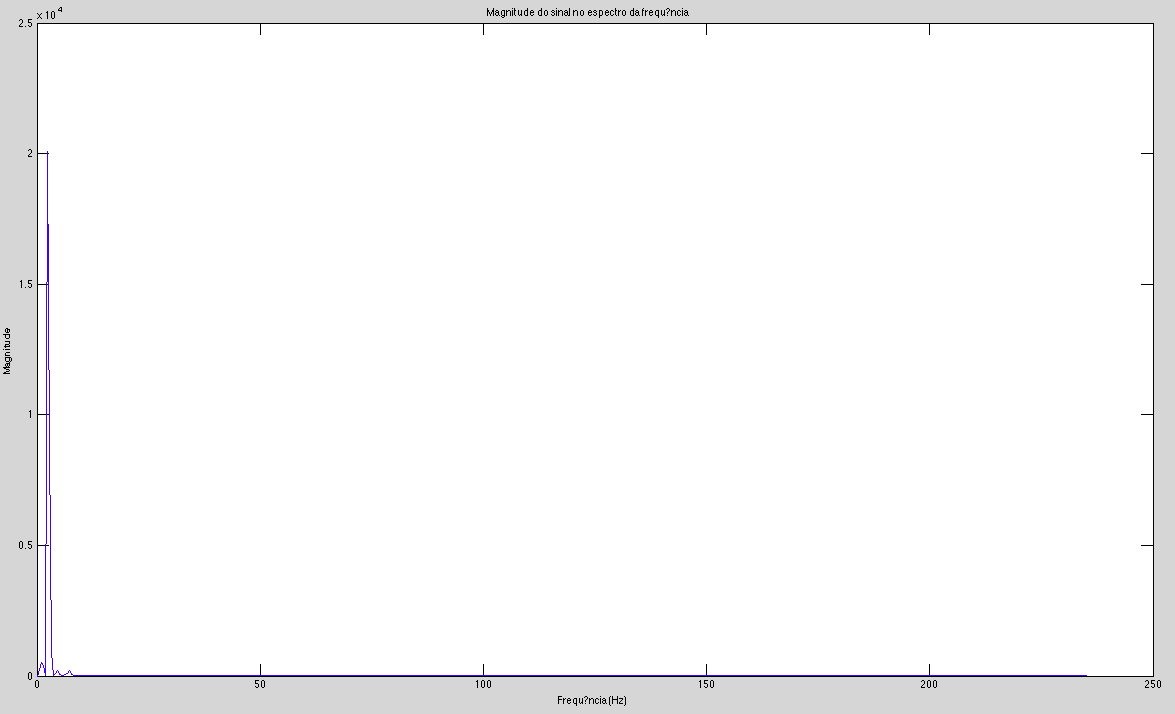
\includegraphics[width=0.47\textwidth]{triangular_fft.png}
        }\\
        \subfigure[]{
            \label{fig:onda_quadrada}
            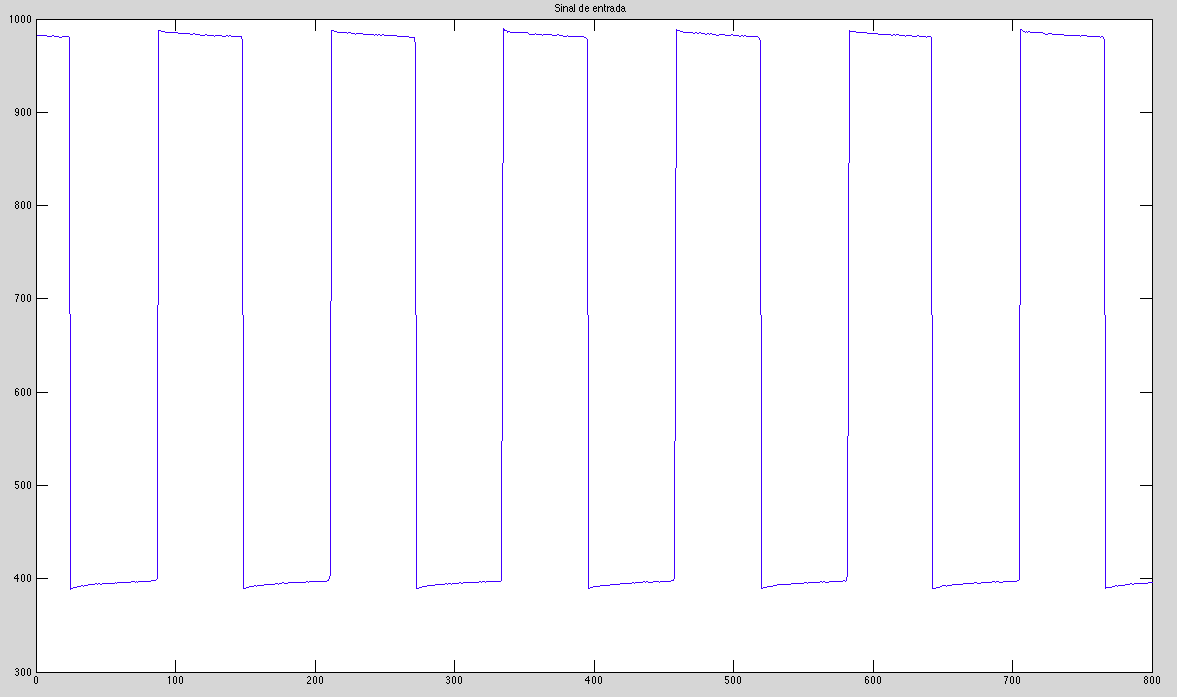
\includegraphics[width=0.47\textwidth]{quadrada.png}
        }
        \subfigure[]{
            \label{fig:onda_quadrada_fft}
            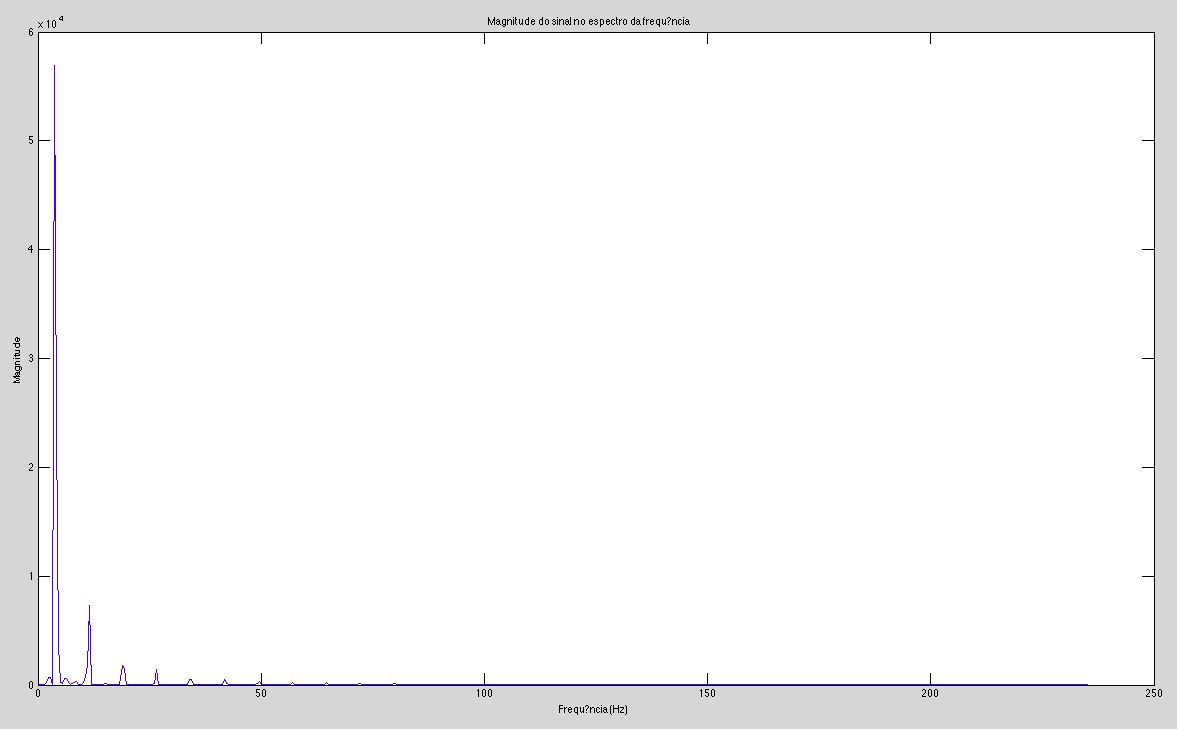
\includegraphics[width=0.47\textwidth]{quadrada_fft.png}
        }
    \end{center}
    \caption{
     	Sinais adquiridos através da solução apresentada: (a) onda senoidal; (c) onda triangular; (e) onda quadrada; e Análise no espectro da frequência dos sinais obtidos: (b) análise do sinal senoidal, (d) análise do sinal triangular; (f) análise do sinal quadrado.
     }
   \label{fig:resultados}
\end{figure}

\begin{thebibliography}{9}

\bibitem{integrationbyexample}
  Boesch, F.,
  \emph{Integration by Example - Euler vs Verlet vs Runge-Kutta}.
  \textit{http://codeflow.org/entries/2010/aug/28/integration-by-example-euler-vs-verlet-vs-runge-kutta/}
  
\bibitem{calculus}
  Leithold, L.; , The Calculus with Analytic Geometry, 6a Ed., HarperCollins Publishers, 1990.

\bibitem{atmega328}
	ATmega328 \textit{http://www.atmel.com/devices/atmega328.aspx}
	
\bibitem{analogdigital}
	Analog and Digital \textit{http://www.stanford.edu/class/cs101/analog-digital.html}
	
\bibitem{transducers}
	What are Transducers? \textit{http://www.wisegeek.org/what-are-transducers.htm}
	
%\bibitem{analogsignal}
%	Analog signal \textit{http://www.princeton.edu/~achaney/tmve/wiki100k/docs/Analog_signal.html}

\bibitem{dsp}
	Processamento Digital de Sinais - Vantagens e Aplicações \textit{http://pt.scribd.com/doc/49815347/Processamento-Digital-de-Sinais-Vantagens-e-Aplicacoes}
	
\end{thebibliography}

\end{document}
